% 使用ctexart文档类(用XeLaTeX编译,直接支持中文)
\documentclass[tikz]{standalone}

\usepackage{pgfplots}
\pgfplotsset{compat=1.10}
\usetikzlibrary{through}

%导言区,可以在此引入必要的宏包

\begin{document} %在document环境中撰写文档
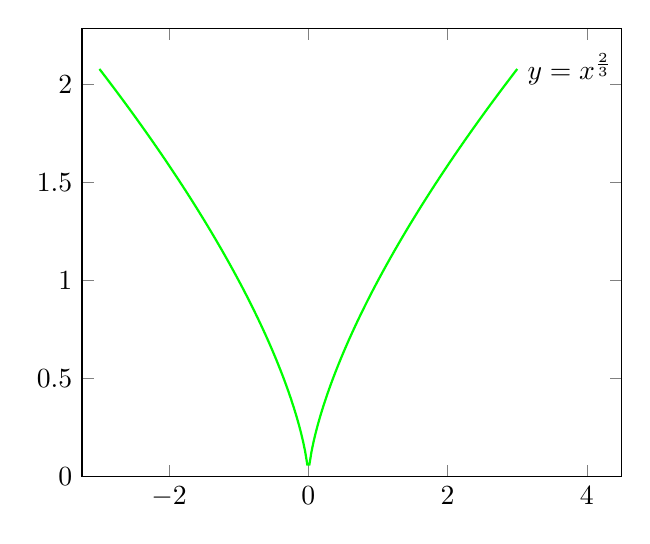
\begin{tikzpicture}
  \begin{axis}[%
      xmin = -3.25, xmax = 4.5,
      ymin = 0,
      domain=-3:3,
      samples=200,
      ]%
      \addplot [green, thick] {abs(x)^(2/3)}node[right,black] {$y=x^{\frac{2}{3}}$};
  \end{axis}%
\end{tikzpicture}%

\begin{tikzpicture}[declare function={f(\x)=pow(abs(\x), 2/3);}]
  \draw[-latex] (-3.25,0)--(4.25,0) node[below] {$x$};
  \draw[-latex] (0,-0.2)--(0,2.5) node[left] {$y$};
  \draw plot[smooth,samples=200,domain=-3:3] (\x,{f(\x)})node[right,black] {$y=x^{\frac{2}{3}}$};
\end{tikzpicture}

\begin{tikzpicture}
  \draw[->] (-3,0) -- (4.2,0) node[right] {$x$};
  \draw[->] (0,-3) -- (0,4.2) node[above] {$y$};
  \draw[scale=0.5,domain=-3:3,smooth,variable=\x,blue] plot ({\x},{\x*\x});
  \draw[scale=0.5,domain=-3:3,smooth,variable=\y,red] plot ({\y*\y},{\y});
\end{tikzpicture}

\begin{tikzpicture}
    \begin{axis}[
        domain=1.037:4,
        xmin=0, xmax=4.5,
        ymin=0, ymax=135,
        samples=800,
        axis lines=center,
    ]
        \addplot+[mark=none,color=green] {5/(x-1)+1};
    \end{axis}
  \end{tikzpicture}

  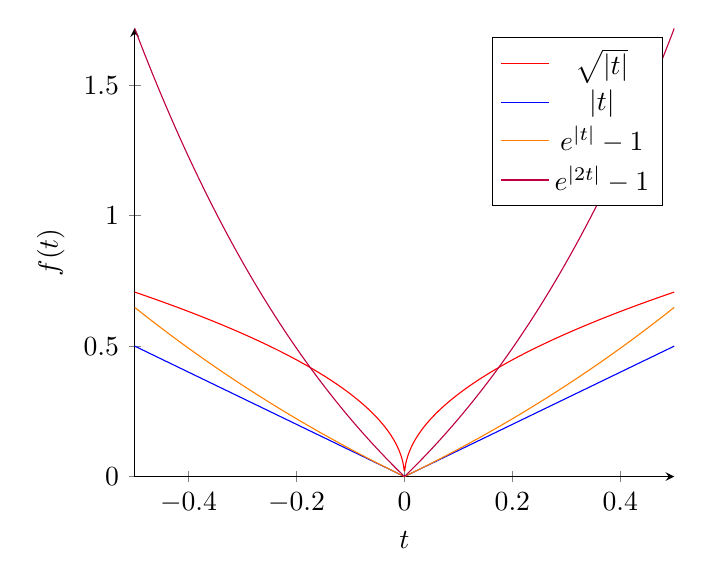
\begin{tikzpicture}
\begin{axis}[
    axis lines = left,
    xlabel = $t$,
    ylabel = {$f(t)$},
]
%Below the red parabola is defined
\addplot [
    domain=-0.5:0.5, 
    samples=1000, 
    color=red,
    smooth,
]
{sqrt(abs(x))};
\addlegendentry{$\sqrt{|t|}$}
%Here the blue parabloa is defined
\addplot [
    domain=-0.5:0.5, 
    samples=100, 
    color=blue,
    smooth,
    ]
    {abs(x)};
\addlegendentry{$|t|$}
%Here the orange parabloa is defined
\addplot [
    domain=-0.5:0.5, 
    samples=201, 
    color=orange,
    smooth,
    ]
    {e^(abs(x))-1};
 \addlegendentry{$e^{|t|}-1$}
 %Here the purple parabloa is defined
\addplot [
    domain=-0.5:0.5, 
    samples=201, 
    color=purple,
    smooth,
    ]
    {e^(abs(2*x))-1};
\addlegendentry{$e^{|2t|}-1$}

\end{axis}
\end{tikzpicture}

\end{document}

%%% Local Variables:
%%% mode: latex
%%% TeX-master: t
%%% End:
